%!TEX root = ../PhDthesis.tex
\chapter{Exploring the role of inhibition in cortical development}

In the previous chapter we explored the spatially calibrated SCAL
model, establishing how various sources of evidence about the spatial
structure of V1 projections relate to each other. While this model was
able to account for the size-tuning properties of the visual cortex
quite well, it also exhibited two major shortcomings. Most importantly
it highlighted that a model lacking distinct excitatory and inhibitory
populations will not be able to capture the diversity in connectivity
and response profiles that are observed in the mammalian
cortex. Secondly we showed that based on the known lack of truly
long-range inhibitory projections, long-range orientation-specific
suppression must be mediated by a di-synaptic mechanism mediated by
long-range excitatory connectivity.

Additionally, in the literature section we described the known
properties of various inhibitory cell classes and what roles they
might perform. In particular we discovered that PV and SOM-expressing
interneurons exhibit highly distinct response properties and
layer-specific expression patterns. With recent techniques enabling
the targeting of specific neural populations, there is now huge
interest in understanding their role both in development and in
mediating and gating both contextual and attentional modulation
phenomena.

In this chapter we will propose a model that incorporate the distinct
response properties of an excitatory pyramidal cell population and the
Parvalbumin expressing interneuron population, allowing us to make
concrete predictions about their role in development. We will
establish that the fast and linear response of the PV-ir, fast-spiking
interneuron population makes them ideally suited towards controlling
feedforward activity, sparsifying activity and thereby driving map
formation. Additionally we will show that this model exhibits more
robust and stable map formation even in the presence of strong lateral
excitation than the previous model.

Specifically we will assess how the model performs when manipulating
the response properties of the PV population, under varying levels of
contrast and strong lateral excitation. The SOM inhibitory population
will be disregarded we are primarily focused on development of the
orientation map, which is known to occur before lateral connectivity
emerges, which is known to drive the SOM interneurons. This inhibitory
cell class will be revisited in the following chapters.

\section{Methods}

\subsection{The SEPI Model}

The \textbf{S}hort-\textbf{R}ange \textbf{E}xcitation \textbf{P}V
\textbf{Inhibition} (SEPI) model is based on the same principles,
spatial profiles and equations that were described for the SCAL model
in the previous chapter. However, unlike SCAL, the model has a
distinct excitatory and inhibitory V1 population, which both receive
afferent input and are connected to each other recurrently. The
architecture diagram (Figure~\ref{SEPIDiagram}) shows the two sheets
and projections between them. When comparing this against the SCAL
model diagram (Figure~\ref{SCALDiagram}), we can see that the
spatial scales of the retinotopy, which generally indicates poor
orientation map organization various projections are unchanged---they
have simply been split up between the populations.

\begin{figure}
	\centering
        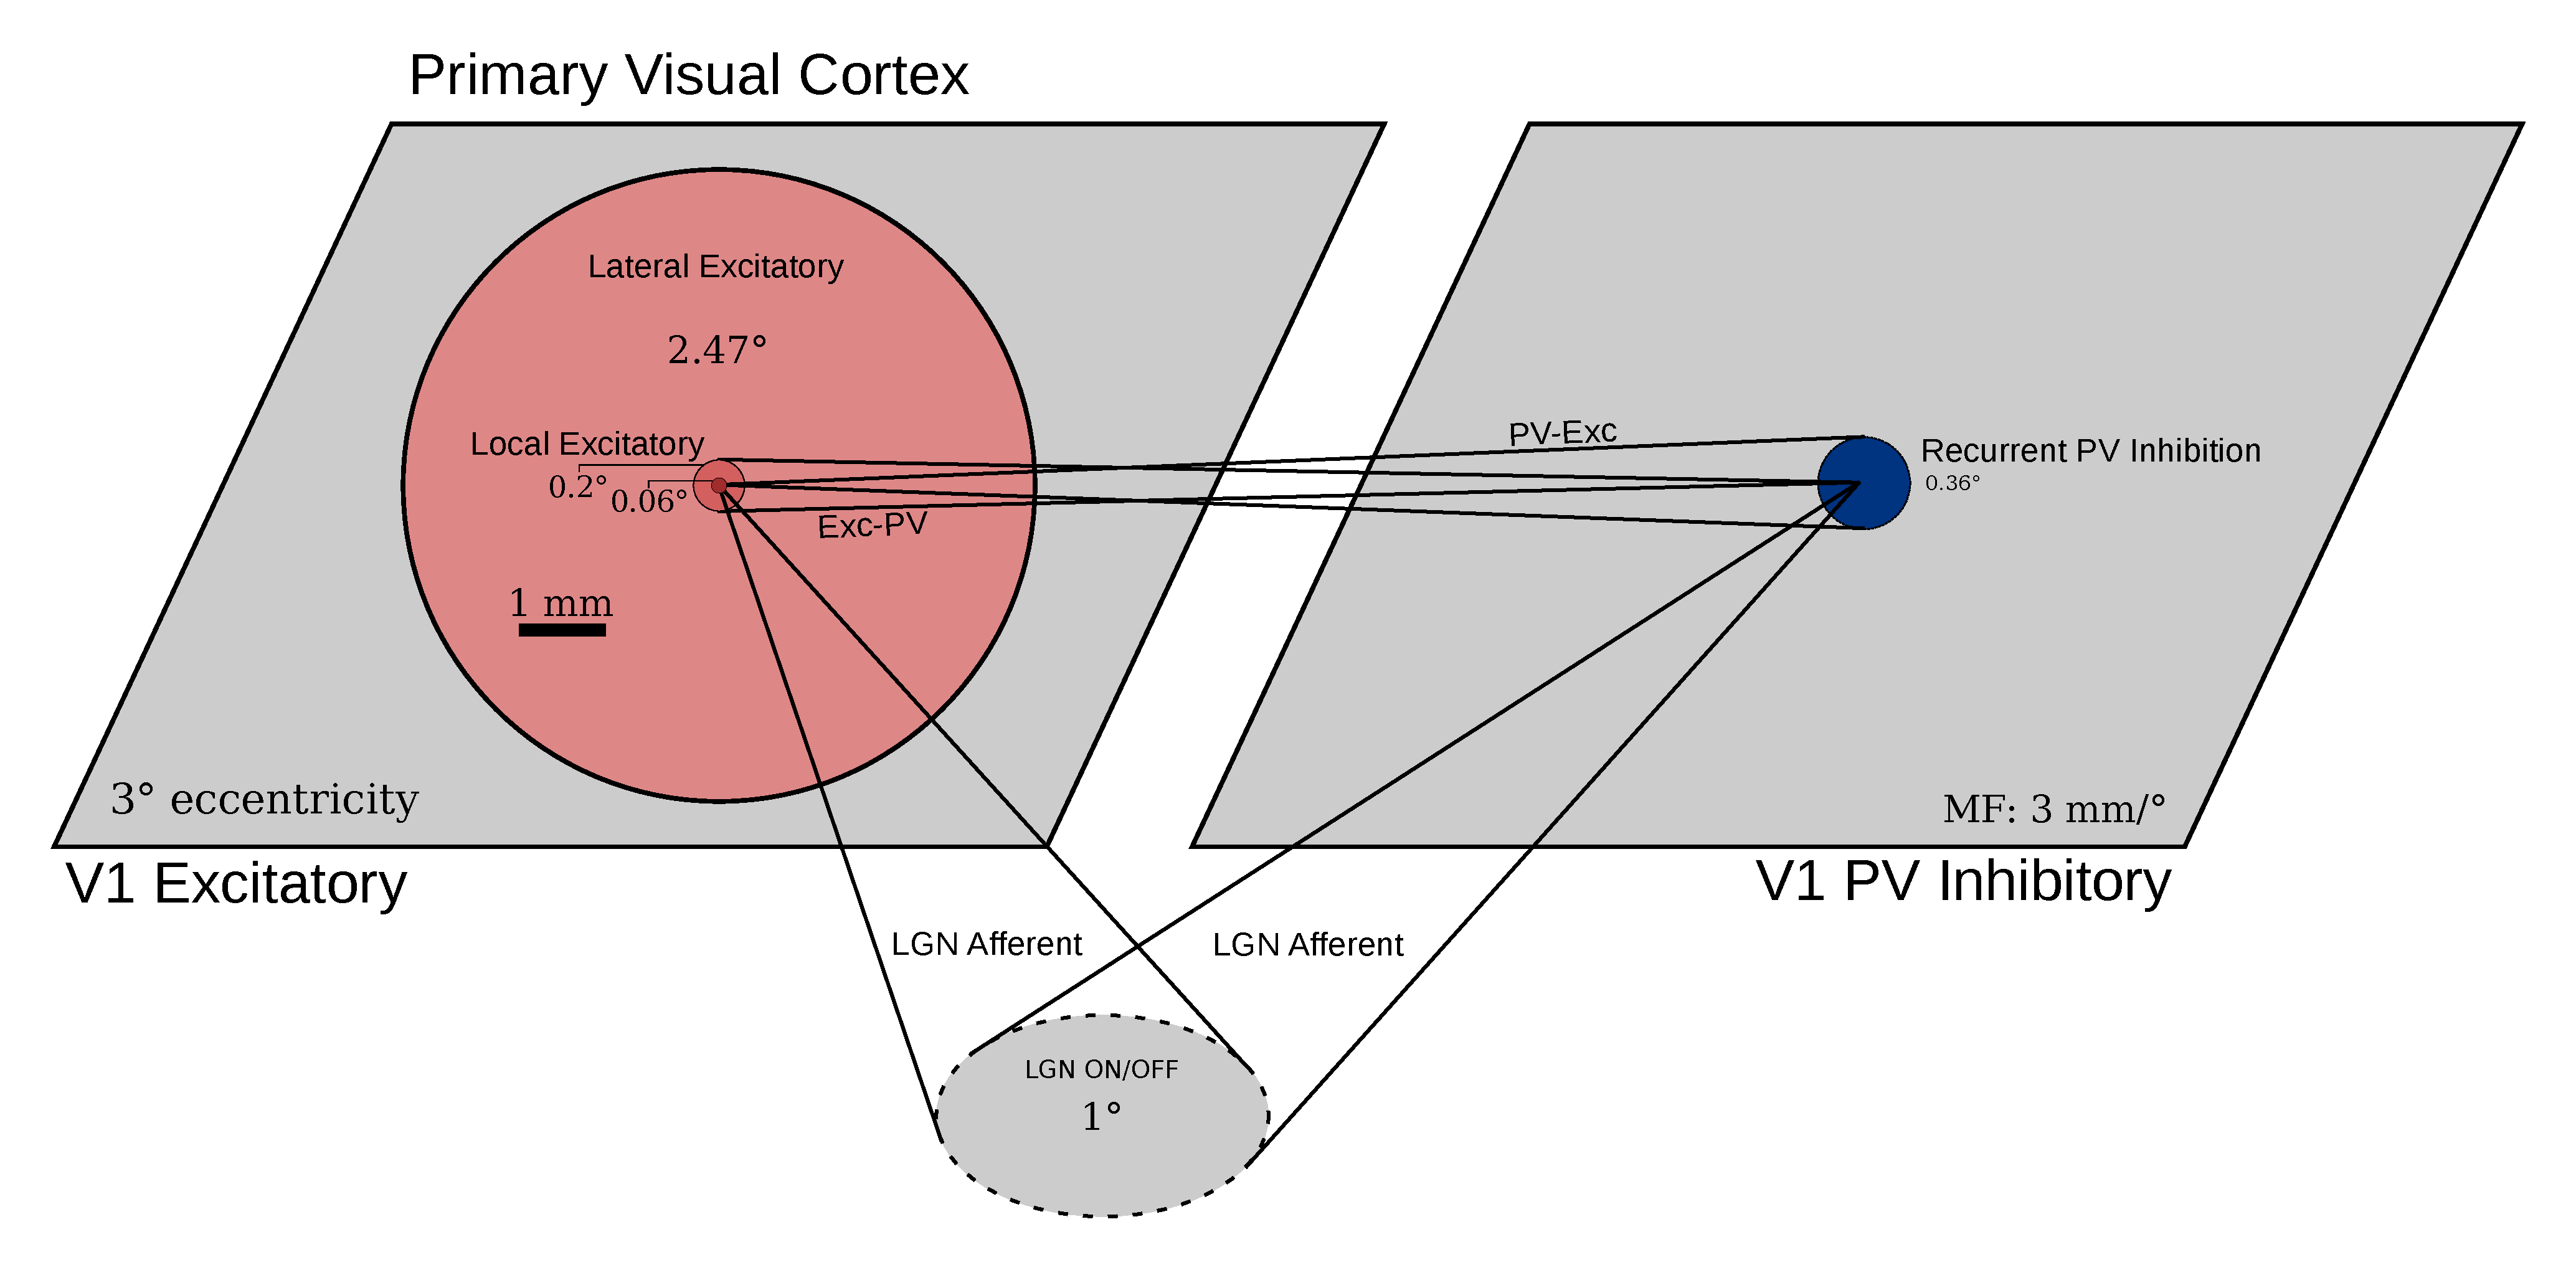
\includegraphics[width=1.0\textwidth]{SEPI_Diagram.pdf}
	\caption{Diagram of the SEPI V1 stage of the model showing the
          spatial scales of the various excitatory (red) and
          inhibitory (blue) connections. Saturated colors indicate the
          kernel radii, while lightly shaded regions indicate kernel
          cut-off extents.}
	\label{SEPIDiagram}
\end{figure}

In the literature review we identified the parvalbumin (PV) expressing
interneurons, which include fast-spiking basket and clutch cells, as
the most likely candidate to provide feedforward inhibition and
controlling the gain of the response in of the pyramidal cells. Their
high abundance in the thalamocortical recipient layer 4 and layers 2/3
(making up over half the population in each;
\citealt{VanBrederode1990}) as well as their involvement in the onset
of the critical period \citep{Fagiolini2000} and their effect on the
columnar organization of the visual cortex \citep{Hensch2004} makes
them of particular interest. The other defining characteristics of the
PV population is their fast response
\citep{Cruikshank2007,Gabernet2005}, and their ability to linearly
match the activity in the excitatory population
\citep{Atallah2012}. These properties describe the role of the
inhibitory projection in the SCAL model, which provides divisive gain
control and is directly coupled to the response of the excitatory
population.

The equations governing the responses of both the excitatory and
inhibitory population are also unchanged, driven by summing the
excitatory input and divided by the inhibitory activity. This closely
matches what we know about PV neurons in the cortex, which provide
strong peri-somatic synaptic inputs to spiny neurons, providing
shunting inhibition \citep{Atallah2012, Wilson2012}. Based on tracing
studies we know that excitatory and inhibitory neurons and
specifically the Parvalbumin expressing subpopulation strongly and
densely innervate each other and themselves \citep{Buzas2001, Ma2011,
  Pfeffer2013}. Additionally these PV population receive strong
afferent input \citep{Burkhalter2008}. All of these properties are
captured by the model.

There is some limited evidence the learning rules on parvalbumin
expressing rules may differ in input cell specific ways with some
anti-Hebbian phenomena having been found in hippocampal circuits
\citep{LeRoux2013}. However for the sake of simplicity the learning
rule applied in the inhibitory population is the same as in the
excitatory population described in equation~\ref{eqn:hebb}.

In order to model the response of the PV population we apply only
half-rectification to the inhibitory population, rather than a
floating homeostatically determined threshold, because basket cells
generally have a very low spiking threshold \citep{Ma2011}.  It would
be possible to use homeostatic plasticity to set the thresholds
instead as suggested by studies in the retina \citep{Hennig2011}, but
it would be complicated to set up mechanisms to balance the thresholds
between the populations to ensure suitable overall levels of activity
in the network. Secondly, we keep the effect of the inhibition
divisive, both for each other and when targeting pyramidal cells.

\subsubsection*{Activation}

The activation for both the excitatory and inhibitory population is
given by:
%%
\begin{equation}
  \eta_E = \eta_I = \frac{\eta_{A} + \eta_{L}}{1 + \eta_{P}}
\label{eqn:sepiactivation}
\end{equation}
%%
where $\eta_{A}$ is the LGN afferent activity, $\eta_{L}$ the local
excitatory contribution and $\eta_{P}$ the PV inhibitory
contribution. In other words, both populations integrate over afferent
and local excitatory input and are then divisively normalized by the
PV population. To allow testing its effects, we will also allow an
optional additional long-range excitation term to modulate the neuron
activity depending on long-range excitatory input:
%%
\begin{equation}
  \eta_{E} = \frac{\eta_{A} + \eta_{L}}{1 + \eta_{P}} (1+\eta_{HE})
\end{equation}
%%
where $\eta_{HE}$ is the input from the horizontal excitatory
projection. The full set of parameters for the SEPI model are list in
Appendix \ref{Appendix:Parameters}. Modeling the long-range input as
an additional multiplicative component has a number of biophysical
explanation, which we will revisit in more detail in the next chapter,
however there is strong evidence that the influence of long-range
excitatory input is strongly voltage dependent \citep{Hirsch1991},
having little effect when afferent input is weak but strongly
modulating the response under stronger input conditions.

The combined activation of the various projections is still combined
in the same way as in the previous models (shown in equation
\ref{eqn:activation1} and as stated above a half-rectifying function
($f$) is used in the inhibitory population, while a homeostatic
function is used among the excitatory population. The response
function of the neurons is therefore given by:

\begin{equation}
\eta_{j,V}(t)=f\left(\frac{\sum_{p=\{E, A\}}\gamma_{p}C_{jp}(t)}{1+\sum_{p=\{I\}}\gamma_{p}C_{jp}(t)}\right)^\beta
\label{eqn:activation2}
\end{equation}

where $\beta$ is the only new term controlling the linearity of the
response, which will be used throughout this chapter.

\subsubsection*{Hysteresis}

In order to control the temporal properties of the PV population we
introduce a hysteresis term, which will be disabled in the final
model but will in the meantime allow us to test the importance of fast
inhibition in the model. The hysteresis function is defined as a discrete
exponential weighting between the previous activation and the new
activity, expressed as:
%%
\begin{equation}
  \eta_h (t + \delta\eta) = \eta(t) + \tau \big[ \eta(t+\delta t) - \eta(t) \big]
\end{equation}
%%
where $\tau$ is the time constant. If $\tau < 1$, hysteresis will
effectively slow down PV responses relative to the excitatory
population. In the final model, the hysteresis term is eliminated simply by
setting $\tau = 1$.

\subsection{Assessing the quality of orientation maps} \label{metrics}

A major component of the analysis applied in this section is to assess
the sensitivity of the model to changes in the response properties of
the different cell classes. Therefore we have to establish a number of
metrics to assess the robustness of the model to changes in contrast
by assessing the quality of orientation map organization.  To measure
the maps, we will focus on the excitatory V1 neurons, though similar
results would be found if we were to pool all the neural types
together as would be the case in optical imaging experiment.  There
are a variety of measures to assess map properties, but we will focus
on four specific measures in particular---smoothness, stability,
selectivity and pinwheel density.

\subsubsection*{Pinwheel density}

Interestingly, it has been found that experimentally measured
orientation maps share a fundamental property across species: pinwheel
count scales linearly with hypercolumn size.  More specifically, there
are $\pi$ orientation pinwheels within the area of one hypercolumn,
when averaging over sufficiently large cortical areas. This
dimensionless, statistical measure of pinwheel distribution is thought
to reflect a universal constant of map organization, converging to
$\pi$ across carnivorans, primates, cats, and tree shrews
\citep{Kaschube2010, Keil2012}. This value was predicted by a
theoretical model of map organization and has strong empirical
evidence, with a mean pinwheel density across four species (tree
shrew, galago, cat, and ferret) statistically indistinguishable from
$\pi$.

Pinwheel density provides such a good measure of map quality because
it is strongly influenced by any number of disruptions of map
organization. Analyzing poor quality maps often reveals other
disruptions in development including poor retinotopy and
selectivity. While it is possible to generate maps which have a
deceptively good pinwheel density metric, this problem can be elimated
by initializing the same model with multiple seeds as was demonstrated
by \cite{Stevens2013}.

To determine the pinwheel density for any given map, the hypercolumn
distance is computed and all pinwheel centers are found. Pinwheel
centers are located at the intersection of the zero contours of the
real and imaginary components in the polar representation of
orientation preference \citep{Lowel1998}. Then we simply divide the
number of pinwheels in the modeled area by the number of hypercolumns
to arrive at the pinwheel density.  \cite{Stevens2013} introduced
pinwheel density as a numerical metric for the biological accuracy of
a map, for which it works well because it has a clear target value.

\subsubsection*{Orientation Selectivity}

When measuring an orientation map using the protocol outlined in
section~\ref{ORMeasurement}, two components are returned. The first is
the orientation preference computed as the vector averaged estimate of
the neurons preference. Additionally there is a selectivity component,
which provides an estimate of how much the neuron will respond to the
preferred orientation relative to all other orientations. This value
provides a simple metric to assess how selective a neuron is, and can
easily be averaged across all neurons in a central region to get an
average selectivity value.

\subsubsection*{Stability}

The stability of orientation maps is determined by determining the
average orientation similarity index of the orientation map over the
course of development. To assess similarity quantitatively,
\cite{Chapman1996} computed the difference of orientation preference
at each developmental age with the organized preference map observed
in the final recording for that animal. As in \cite{Stevens2013} we
normalize these similarity values to fall between 0 (completely
uncorrelated) to 1 (identical orientation preference). The orientation
similarity index is therefore defined as:
%%
\begin{equation}
  OSI = 1 - \frac{4}{n\pi} \sum_{i}\abs{(F_{i}-O_{i})\bmod\frac{\pi}{2}}
\end{equation}
%%
where $i$ iterates over each neuron in the orientation map $F_i$
represents the final orientation preference and $O_i$ is the
orientation preference at an earlier time. By averaging the OSI at
every 1000 development steps we can numerically compare the stability
of the model over time, which provides a measure of how quickly and
how smoothly the map is becoming organized. Note that there is no
objective criterion for ``best'' stability, since a perfectly stable
map that never achieves selectivity would be a failure both as a model
and as a visual system, but in conjunction with other measures the
stability metric is helpful for evaluating the effect of changing
specific parameters for a given model.

\subsubsection*{Local Homogeneity Index}

The local homogeneity index (LHI) was first introduced by
\cite{Nauhaus2008} as measure of the local smoothness of the map. It
is therefore useful to determine whether a neuron is in a smooth
region of the orientation map or near a pinwheel region where the
orientation preference varies considerably. The LHI is defined based
on a specific $\sigma$ value, which should reflect the spatial
properties of the map. Therefore we can use the mean LHI across the
entire map as a measure of the scale of homogeneous regions of the
map. The LHI at location x is computed as follows:
%%
\begin{equation}
  LHI(x) = \frac{1}{2\pi \sigma^2} \bigg\lvert \int
  exp\bigg(\frac{-\|x-y\|^2}{2\sigma^2}\bigg) exp(i2\theta_y) dy
  \bigg\rvert
\end{equation}
%%
where $\theta_y$ is the orientation preference at site y and $\sigma$
determines the spatial scale of the analysis. In their experiments
\cite{Nauhaus2008} used $\sigma=180\mu m$ to match the spatial extent
of dendritic fields in both cat and monkey cortex.

\subsubsection*{Center-of-Gravity Distortion}

Since we have access to all the weights in the model, we can easily compute
the center-of-gravity (CoG) of the afferent weights relative to the
position of the neuron, to determine how far the neuron's preferred
location is from its perfectly retinotopic mapping.  Some retinotopic
distortion will always be present, due to locally smooth organization
for features like orientation, but extreme distortions are not typical
for biological maps, and are thus an indication of inappropriate
parameter settings or training patterns for a model network.

The CoG along one axis is computed as the mean of the normalized
vector product: 
%%
\begin{equation}
  G(p, \omega) = \frac{1}{\sum_{i,j} \omega_{i, j}} \sum_{i,j} \omega_{i,j} p_{i,j}
\end{equation}
%%
where $p$ is the position along either the x- or y-axis and $\omega$
is the weight at that location. The distortion in the CoG is then
given by Euclidean distance between the center of gravity and the
actual retinotopic location of the neuron:
%%
\begin{equation}
  G_d(x, y) = \sqrt{(CoG_x-x)^2 + (CoG_y-y)^2}
\end{equation}
%%
By computing this distance for all neurons in a central region, we can use
this metric as a measure of the quality of the retinotopic mapping in
the model, highlighting any distortions.

\section{Results}

In this section we will present results analyzing the results from
both the SCAL and SEPI models. First establishing the role of
inhibitory neurons in development in the SEPI model and then comparing
how robust the models are to varying levels of contrast and long-range
excitation. These results will primarily be based on four different
metrics the local homogeneity index (LHI), orientation selectivity,
stability, Center-of-Gravity distortion and pinwheel density.

Before using these metrics to evaluate the different models it is
important to understand what they actually measure and how it relates
to the quality of the model. The pinwheel density is the only
scale-free measurement and has been discussed sufficiently in the
previous chapter. The other metrics are shown for each unit in the
model in Figure~\ref{MetricPlots} and will be averaged to get a single
value to assess the model.

\begin{figure}
  \includegraphics[width=1.0\textwidth]{./results/sepi/Metrics.pdf}
  \caption[Metrics used to evaluate orientation map
    development.]{Metrics used to evaluate orientation map development
    taken from a $2x2^\circ$ region in the model. A) Local homogeneity
    index representing how similar neurons in a local region are, poor
    organization will lead to large high-homogeneity regions or low
    global homogeneity. B) Orientation selectivity measures the
    overall selectivity of the neurons. Low mean selectivity indicates
    poor and unstable development. C) Stability measures the
    self-similarity of the orientation preference over time. Low
    stability, i.e. values well below 0.8, values indicate continuous
    reorganization of the orientation map. D) Center-of-gravity
    distortion represents a measure of how precise the retinotopy in
    the model is. Significant amounts of CoG distortion indicates poor
    retinotopy, which generally indicates poor orientation map
    organization.}
	\label{MetricPlots}
\end{figure}


\subsection{Development}

The role of inhibition in development is hugely important, as
evidenced by the fact that a variety of pathological conditions
including autism \citep{Wohr2015} and schizophrenia \citep{Lewis2012}
have been tied to changes in PV-expressing interneurons in the
cortex. Modeling the role of these cell classes in development and
adult visual processing requires accurately modeling their response
properties. Since the synaptic projections develop as a result of
these properties, the tuning properties of the modeled neurons in the
developed model will let us make concrete predictions about the role
of these neurons in shaping V1 development.

Accurately capturing the response of these neurons in a rate-based
model presents a number of challenges because we cannot explicitly
model fast-spiking kinetics, which means we are limited to modeling
higher absolute firing rates. Additionally, much of the data about
these cell classes comes from mouse experiments, because of the new,
rich techniques for genetic manipulation of specific cell classes,
rather than primates or carnivorans as for most of the functional
data.

The spatial extent of the PV neurons was already calibrated for the
SCAL model, and so the next step is to calibrate their inputs and
response properties. The literature is very clear that PV neurons in
the visual cortex receive strong inputs both from thalamocortical
afferents and from recurrent inputs, so the main question to settle is
how closely these neurons are coupled to the excitatory population. It
has been hypothesized that these neurons can quickly and robustly
balance out the excitation arriving from the LGN \citep{Swadlow2003,
  Burkhalter2008}, by linearly matching the response of the pyramidal
cell population and providing contrast gain control to sparsify the
activity and thereby sharpen the orientation tuning
\citep{Wilson2012}.  If so, then a non-linear and very slow response
among this population should disrupt map development, which is a
prediction that we will test in the model.

\subsubsection*{Linearity and time profile of inhibitory responses}

To help understand how the PV population affects the behavior of the
model, variants of the model were launched using different PV
activation functions determined by two parameters. The parameter
determines the linearity of the response, by adding an exponential
term after the half-rectifier defined as the $\beta$ term in equation
\ref{eqn:activation2}. By varying this exponential term we could vary
the response of the neuron from sub- to supra-linear values. To
control the time profile of the response, a hysteresis term was added
as well. After training, these model variants were assessed based on
the metrics outlined in Section~\ref{metrics}.

\begin{figure}
	\centering
        \includegraphics[width=1.0\textwidth]{./results/sepi/SEPI_Linearity.pdf}
	\caption[Analysis of development in SEPI model when varying time
      constant and linearity of responses]{Parameter exploration to
      determine how the linearity and time constant of inhibitory
      responses affect development. A) A measure of stability of the
      model over time, integrating the similarity index of the model
      over time. B) Orientation selectivity in the model measured
      using orientation map measurements. C) The average local
      homogeneity index measuring the smoothness of the map at a
      particular spatial scale. D) Pinwheel density of the model,
      which should approach $\pi$ for a perfect map. E) The
      Center-of-gravity (CoG) distortion provides a measure of how
      much the retinotopy in the model has been disrupted. The color
      mapping was chosen to match Figure \ref{MetricPlots} and
      simplify comparison. The model maps match biological results
      only when the PV exponent is 1 (linear response) and does not
      respond too slowly.}
	\label{SEPILinearity}
\end{figure}

The results of the parameter exploration are shown in figure
\ref{SEPILinearity}. They include a measure of stability over time,
orientation selectivity, distortion of the retinotopy, the mean local
homogeneity index (LHI) and finally the pinwheel density ($\rho$),
used to assess the quality of the maps.

The immediately striking result is the narrow band of good (i.e., near
$\pi$) pinwheel densities in the linear region of the response. Apart
from that, we can clearly see that orientation selectivity, stability
and the CoG distortion are strongly correlated with each other and all
anti-correlated with the LHI. In particular, we can see increasing
distortion of the retinotopy as the inhibitory population responds
more strongly, which causes serious disruptions to the map quality. At
the same time, sub-linear responses lead to very weak selectivity,
which causes relatively low stability and high homogeneity.

In order to get a better overview of the relationships between these
variables, Figure~\ref{SEPILinearityCorr} shows the correlation matrix
between the independent variables we are exploring and the
metrics. The results highlight once again the strong relationship
between orientation selectivity, stability, and the CoG shift and
supra-linear PV cell responses. This view makes it clear that the PV
cell exponent has a much greater effect on the various metrics than
the time constant of the response, which does not show significant
effects until the response is very slow.

\begin{figure}
	\centering
    \includegraphics[width=0.7\textwidth]{./results/sepi/SEPI_Linearity_Correlations.pdf}
	\caption{A correlation matrix of the various dependent and
      independent variables when varying the linearity and time
      constant of PV neuron responses. Plots the Pearson correlation
      of the various metrics with each other, showing how these
      metrics are related. Highlights the strong correlation between a
      super-linear response and high selectivity, stability and
      retinotopic distortions.}
	\label{SEPILinearityCorr}
\end{figure}

Overall we can conclude that a linear response, but not necessarily a
very fast response, is required to drive the development of a
high-quality orientation map. We will attempt to disentangle the
causal relationships between these variables in the
discussion. Meanwhile, however, we have a strong claim that we can develop
high-quality orientation maps in the model. As a next step we will
investigate how this model compares to the SCAL model.

\subsection{The SEPI Model}

The idea behind developing a model with distinct excitatory and
inhibitory populations was based on three main observations. The first
is straightforward: we know that in biology a single class of neurons
will essentially never provide excitation at some synapses and
inhibition at others, a principle known as Dale's law. From this
perspective the SEPI model already provides an advantage over the SCAL
model, showing how SCAL could be implemented in neural
circuitry. However we also wanted to see whether this model could
improve the diversity in responses and more accurately capture
contrast-dependent responses in the model, while continuing to develop
high quality maps and exhibiting robust and stable self-organization.

\begin{figure}
	\centering
    \includegraphics[width=1.0\textwidth]{./results/sepi/SEPI_V1_ORTuning.pdf}
	\caption{SEPI model orientation tuning properties after presenting
      20,000 oriented Gaussian patterns. A) Orientation map measured
      by presenting sine gratings at the optimal spatial frequency to
      the model, along with the locations of the receptive fields
      shown in B. B) Gabor-fits to receptive fields measured using
      sparse random noise. C) Orientation tuning curve of a single
      excitatory neuron across contrasts, demonstrating largely
      contrast-independent orientation tuning. D) Orientation tuning
      curve of a PV neuron displaying a weakly tuned response, with a
      certain baseline of activity which is only weakly modulated by
      orientation.}
	\label{SEPIORTuning}
\end{figure}

The linearity analysis already confirmed the model could produce
high-quality orientation maps. In \ref{SEPIORTuning} this is further
confirmed with a high-quality map, and clearly defined receptive
fields, which exhibit contrast invariant orientation tuning, which
rivals previous models. Without going into detail, we can also confirm
that the spatial calibration still holds, with ~3.5 cycles per visual
degree, well within the acceptable margins that were established in
Figure~\ref{SCALHypercolumns}.

\begin{figure}
	\centering
        \includegraphics[width=0.8\textwidth]{./results/sepi/SEPI_V1_DoG_Contrast.pdf}
	\caption{Contrast-dependent shifts in size tuning as estimated by
      the DoG model. A) Spatial constant of the excitatory center of
      the DoG model at low vs. high contrast. B) Distribution of
      contrast-dependent shifts, showing a much better match to the
      experimental data than GCAL or SCAL (see figure
      \ref{ContrastShift}).}
	\label{SEPI_DoG_Contrast}
\end{figure}

The main thing we are interested in, however, is how decoupling the
two populations affects contrast-dependent size-tuning shifts, which
rely on strong divisive inhibition. Recall for example that the GCAL
model showed very little contrast-dependent size-tuning changes due to
the inhibition being purely subtractive. The SCAL model demonstrated a
strong shift, but it lacked the diversity observed in the experimental
data. Repeating this same protocol in the SEPI model as is shown in
figure \ref{SEPI_DoG_Contrast}, demonstrates a slightly larger shift
in contrast-dependent size tuning, which is in fact exactly in line
with other measurements performed in macaque ($\approx
2.2\times$). Even more strikingly, the model now exhibits diversity in
size tuning shifts that provide a far better match to experimental
results (Figure~\ref{ContrastShift}). This likely can be attributed to
the greater strength and variation of inhibition that is made possible
by partially decoupling the excitatory and inhibitory population.

Introducing a separate inhibitory population also allows us to compare
the spatial and orientation profile of inhibitory neurons more
realistically, since they no longer reflect the activation of the
joint excitatory/inhibitory population. When comparing
Figure~\ref{SEPI_OR_Distributions} to \ref{LatORDist} we can see that
the neurons are no longer as strongly biased toward the preferred
orientation of the excitatory neuron, which is a direct result of much
broader orientation tuning in the inhibitory PV
population. Additionally the inhibitory connections seem to exhibit
longer tails, particularly in the oblique and cross-orientation
distributions, which more closely matches the experimental data. The
major difference when compared to the experimental data seems to be in
the relative weights of connections targeting iso-, oblique- and
cross-orientation domains. Since the model distributions represent the
actual weights while experimental data just uses the total count of
boutons it is unclear whether this difference arises simply because it
is not possible to accurately measure connection strengths in
experiments. Overall these orientation distribution of inhibitory
connections in the SEPI model more closely reflects the experimental
data when compared to the SCAL model.

\begin{figure}
	\centering
    \includegraphics[width=1.0\textwidth]{./results/sepi/SEPI_Inh_OR_Distributions.pdf}
	\caption{Spatial distribution of weights targeting A)
      iso-orientation regions, B) oblique-orientation regions and C)
      cross-orientation regions. Inhibitory neurons in the SEPI model
      have a much broader distribution of connections in the
      orientation domain, more closely matching \cite{Kisvarday1997a}
      than the SCAL model.}
	\label{SEPI_OR_Distributions}
\end{figure}

Finally, we can confirm the spatial and orientation tuning properties
of the SEPI model in another way. By computing the local homogeneity
index as we did above, we can compute the smoothness of the map at a
specific spatial scale. Since we know the spatial scales in the model,
we can directly compare the distribution of the LHI to experimental
data. The $\sigma$ value was therefore set to $180 \mu m$ and plotted
against the orientation tuning width of all neurons in a central
region of the simulated map. The resulting scatter plot is shown in
Figure~\ref{SEPILHI}, compared directly to equivalent measurements in
macaque and cat visual cortex. Both the distribution of tuning widths
and LHI values closely match the experimental data from macaque, but
not cat, which is exactly what was desired.

\begin{figure}
	\centering
        \includegraphics[width=0.6\textwidth]{./results/sepi/SEPI_LHI.pdf}
	\caption{Local homogeneity index against tuning width in the SEPI
      model compared to experimental results from macaque monkey and
      cat. Reproduced from \cite{Nauhaus2008}. Provides another
      confirmation of appropriate spatial calibration, as the LHI is
      dependent on the scale of orientation columns.}
	\label{SEPILHI}
\end{figure}

While the model now exhibits many of the properties that were lacking
in the SCAL model, one last issue remains. A large reason why the SEPI
model was introduced in the first place was to come up with a model
that would exhibit realistic long-range connectivity, which is
presumed to underlie various contextual modulation effects. In this
next section the effect of introducing long-range excitatory on the
development of the model will be explored to see whether this model
can robustly develop even in the presence of the long-range patchy
connections that are so characteristic of pyramidal cells in layer 2/3
of the cortex.

\subsubsection*{Robustness to long-range excitation}

At this point two separate but very similar models have been
introduced, SCAL and SEPI, which differ mostly in that the latter has
distinct excitatory and inhibitory populations. The major reason why
the populations were split in this way is to match the anatomy, but
does this change actually buy us anything from a functional
perspective? In order for long-range excitation to mediate contextual
modulation phenomena, these projections need to be able to
meaningfully modulate neuron activity at long distances. However, from
a theoretical perspective, introducing strong long-range excitatory
connectivity in a model seems problematic for a number of reasons. The
most obvious and problematic result of strong excitation is that it
can lead to runaway, `epileptic` activity in the cortex, which results
in severely disrupted development as we already saw when inhibitory
neurons responded sublinearly. More subtly however, by introducing
long-range correlations into the activity we can disrupt the
retinotopy in the model and violate the sparse coding hypothesis,
which have been shown to play crucial roles in self-organization.

Therefore assessing how the models hold up in the presence of strong
lateral excitation under varying contrast levels will help us
establish how robust the model is and lay the groundwork for a model
that exhibits both long-range excitation and suppression. Thus we will
compare how the SCAL and SEPI models deal with varying levels of
contrast and lateral excitation to investigate whether separating the
populations has any benefits in addition to being more anatomically
realistic.

\paragraph{SCAL}

\begin{figure}
	\centering
        \includegraphics[width=1.0\textwidth]{./results/SCAL/SCAL_Robustness.pdf}
	\caption{Parameter explorations of three separate metrics of
      orientation map development using the SCAL model from
      Chapter~\ref{SCALmodel}. Plotted on $x$ and $y$ are the strength
      of long-range lateral excitation and the stimulus contrast
      during training. The metrics show \textbf{A} the orientation map
      stability metric, \textbf{B} the average selectivity over the
      time course of development, \textbf{C} the average local
      homogeneity index providing a measure of map quality, \textbf{D}
      the $\rho$ pinwheel density metric, which characterizes the
      quality of the map, and \textbf{D} the mean amount of
      Center-of-Gravity distortion providing a measure of retinotopic
      distortions. The model is highly robust to varying stimulus
      contrasts at low levels of lateral excitation, but quickly
      deteriorates with increasing levels of excitation.}
	\label{SCALStability}
\end{figure}

The results of this analysis, once again assessed by the list of
metrics described above, are shown above in \ref{SCALStability}. The
first thing to note is that increasing lateral excitation leads to
immediate disruptions to the self-organization of the model until we
reach a transition point at which the model fails to self-organize
completely, presumably the point where the additional excitation can
no longer be balanced by increases in the gain of inhibition. Indeed,
the CoG distortion increases with increasing lateral excitation,
suggesting that activity is allowed to propagate horizontally from
where it arrives in V1, leading to disruptions in retinotopy. Overall,
we can see that adding strong lateral excitation to SCAL causes
disruptions to the stability, orientation selectivity, pinwheel
density, and CoG distortion, causing the eventual breakage of the
entire model.

The correlation matrix shown in Figure~\ref{SCALRobustnessCorr}
highlights what is going wrong as we increase the lateral
excitation. It demonstrates a strong relation to CoG distortion and
increasing homogeneity, with clear anti-correlation with orientation
selectivity and stability. As a result we can conclude that the
lateral excitation leads to disruptions in retinotopy and lower
selectivity, which in turn disrupt the stability and pinwheel density
of the model.

\begin{figure}
	\centering
    \includegraphics[width=1.0\textwidth]{./results/SCAL/SCAL_Robustness_Correlations.pdf}
	\caption{A correlation matrix of the various dependent and
      independent variables of the linearity analysis. Plots the
      Pearson correlation of each variable against each other
      variable, for the SCAL model from Chapter~\ref{SCALmodel}.}
	\label{SCALRobustnessCorr}
\end{figure}

\paragraph{SEPI}

When applying the same analysis to the SEPI model
(Figure~\ref{SEPIStability}), we can immediately see that the model
shows very little disruption at equivalent levels of lateral
excitation.  The model shows basically no CoG distortion, and very
little variation in pinwheel density, stability, and LHI. The
orientation selectivity, conversely, actually increases with both
excitation and contrast, opposite to what was observed in SCAL. Of
course, even this model begins to break down under very high contrast
and strong lateral excitation.

\begin{figure}
	\centering
        \includegraphics[width=1.0\textwidth]{./results/sepi/SEPI_Robustness.pdf}
	\caption{Parameter explorations of three separate metrics of
      orientation map development using the SEPI model. In comparison
      to the SCAL model, the model is far more robust to strong
      lateral excitation and maintains almost uniform stability across
      almost all explored parameter values. As in
      Figure~\ref{SCALStability} panel \textbf{A} shows the
      orientation map stability metric, \textbf{B} the average
      selectivity over the time course of development, \textbf{C} the
      average LHI providing a measure of map quality, \textbf{D} the
      $\rho$ pinwheel density metric and \textbf{D} the mean CoG
      distortion. Uncoupling of excitation and inhibition allows the
      model to handle changes in parameter strengths in a robust and
      responsive way.}
	\label{SEPIStability}
\end{figure}

Overall, however, the SEPI model is significantly more robust to
variations in the strength of afferent input and even lateral
excitation, which is usually thought to cause problems for models
that rely on competition between neurons to represent the visual
space.

\section{Discussion}

In this chapter we have explored how distinct excitatory and
inhibitory modeled after the pyramidal and basket cells in the visual
cortex interact to give rise to robust and stable map formation and
then confirmed the model still matches the other spatial and
orientation tuning properties we carefully evaluated in the SCAL
model.

\subsection{The role of inhibition in development}

In the first experiment we asked what happens when we decouple the
responses of the inhibitory population from that of the excitatory
population. In the SCAL model and all most previous SOM based models
both excitatory and inhibitory cells were represented by the same
neurons, which means their responses were coupled directly. While the
time constant had very little effect on the organization of the model,
the analysis highlighted how strong an effect a non-linearity in the
activation function of the inhibitory population had. A sub-linear
response was associated lower selectivity and stability, while a
supra-linear response was associated with very high orientation
selectivity but also greater distortion in the retinotopy.

From a theoretical perspective these results make sense: a linearly
responding PV population is able to match the level of excitation that
is arriving in the cortex from thalamocortical afferents and recurrent
intra-cortical connections; shifting that balance in either direction
will disrupt the development. Indeed, if we compare the effect of
up-regulating the PV responses, we can see some parallels to what
happens during pharmacological up-regulation of $GABA_A$ neurons by
administering the $GABA_A$ agonist benzodiazepine (diazepam)
\citep{Fagiolini2004,Hensch2004} and looked at ocular dominance
columns rather than orientation columns. Much like in those
experiments, the neurons become more segregated and selective when the
inhibitory population was up-regulated in this way. The results
predict that the orientation column spacing narrows with increasing
inhibition, which does not match the results obtained for ocular
dominance columns. This may be explained by the fact that the
development of ocular dominance columns precedes that of an
orientation map, and the diffuse and unorganized initial pattern of
GABAergic connections acts to patches of correlated activity further
apart rather than concentrating it in a smaller column.

The hysteresis term in the responses of PV neurons was not used in the
final model for two reasons. Firstly it had little effect on the
organization of the model unless very low time constants were used
resulting in highly sluggish responses and potential decoupling of the
excitatory and inhibitory populations. Additionally since this
population is modeled after the fast-spiking population, which exhibit
fast very fast kinetics \citep{Cruikshank2007,Gabernet2005}, a more
instantaneous reponse fits more closely with our experimental
observations about this population of interneurons.

Finally, we compared how the SCAL model compared to the SEPI model in
terms of robustness to lateral excitation and varying levels of
contrast. These results clearly showed that the SEPI model
self-organizes for a much wider range of lateral excitation values,
indicating it can deal with the destabilizing introduction of
long-range excitation much better. This property is likely a direct
result of separating the two populations. Although separating the
populations allows these neurons to become uncoupled, it also ensures
that the inhibitory population can effectively respond and cancel out
the additional excitation arriving via long-range connections. In this
way high activity among the excitatory population results in more
effective suppression rather than complete destabilization of the
network. However, at the very highest lateral excitation and contrast
values tested here, even this model had trouble canceling out this
additional excitation.

Based on the overall observations, it seems that the model's PV
population provide a means for the neurons in a local region to
compete to represent the stimulus, repelling neurons with similar but
somewhat different feature preferences.  This process results in a
smooth local mapping of the feature preferences into an orientation
map. Having neurons that respond so quickly and robustly ensures the
development of a realistic orientation map even in the presence of
other influences, though it also means that pathological changes in
the PV response properties could severely disrupt the organization of
the cortex.

\subsection{Feature tuning and inhibition}

When analyzing the model size and contrast response, we found very
good agreement with experiment, and even found that the variability in
responses was much more realistic compared to the SCAL model. By
decoupling the excitatory and inhibitory neurons, we were able to
achieve a greater contrast-dependent size-tuning shift, both
qualitatively and and quantitatively much closer to the kinds of
shifts that are seen in experiment (see Figure~\ref{SEPI_DoG_Contrast}
and \ref{ContrastShift}). This result fits very well with the idea
that the PV neurons exert strong control over the response gain of
principal neurons via a divisive mechanism \citep{Wilson2012}. Indeed,
through artificial up-regulation of the PV population, not currently
shown, we could mirror the effects of decreasing the contrast,
matching results found by \cite{Nienborg2013} in mouse visual cortex.

One major question in the literature has been the tuning properties of
PV neurons. A number of theoretical studies had suggested that untuned
or broadly tuned inhibition in the visual cortex was required for the
development of orientation selectivity or its contrast invariance
\citep{Somers1995, Troyer1998}. The work by \cite{Cardin2007}
challenged this assumption, because they found that the fast-spiking
inhibitory cells in layer 4 of cat area 17 did not exhibit
significantly broader tuning in the subthreshold response than the
regular spiking excitatory population. However, they did find broader
tuning in the spiking response in this population, and similar studies
had found conflicting results \citep{Hirsch2003, Nowak2008}. In the
SEPI model, the PV cells generally display orientation tuning, but
they are overall significantly more broadly tuned than the excitatory
population, which is largely driven by the fact that the modeled cells
do not have any spiking threshold. \cite{Cardin2007} argue that
studies such as \cite{Nelson1994}, which demonstrated no widening in
orientation tuning of excitatory cells under GABAergic inactivation,
suggest that broad inhibitory tuning does not significantly contribute
to sharpening of orientation tuning. However, this argument ignores
the role of inhibitory neurons in shaping the responses and tuning of
neurons during development, such that the instantaneous responses of
the inhibitory population are no longer needed to significantly
sharpen the tuning of excitatory cells, as their tuning has already
been encoded in the feedforward connections (as noted by
\citealt{Miikkulainen2005}).

Another difficulty is in determining layer-specific effects; e.g.,
\cite{Cardin2007} primarily measured from fast-spiking cells in layer
4. It may be the case that fast-spiking neurons in layer 4 are more
closely involved in a push-pull inhibitory regime, which would require
sharper orientation tuning \citep{Hirsch2003, Hirsch2006a}. Further
investigation will be required to determine the precise properties of
the PV-ir neuron population across layers in species with maps, in
order to determine whether there are functionally distinct subgroups.

\subsection{Conclusion}

Overall, the results here indicate that the PV population is very well
suited towards mediating the kinds of tasks that are important for
robust development. Specifically, they can linearly track the
responses of pyramidal cells in their vicinity by integrating
feedforward and recurrent input and matching the levels of excitation
in these neurons. Including PV neurons leads to a model that is highly
robust to long-range excitation, but still exhibits all the desirable
properties of the SCAL model, including contrast-invariant orientation
tuning and the same spatial tuning.

At the same time, however, the model still has no way of mediating any
true long-range orientation specific inhibitory effects. This is
because the PV neurons are very broadly tuned and if allowed to
develop only receive very weakly tuned long-range excitatory
connections. Additionally, due to the strong inputs they receive and
their internal dynamics, PV neurons are very fast in their response
and adapt very quickly, making it difficult to envision how they could
integrate activity that arrives over longer spatial and temporal
scales.
